% Shared body for the IEEE and ACM builds. Numbers in this file come from results/*/copy.json
% via paper/make_figures.py; update both together.

\section{Introduction}

Long-context modeling has become a headline feature of DNA language models (DNA~LMs).
HyenaDNA~\cite{nguyen2023hyenadna} reports checkpoints with context windows up to 1\,Mbp,
Caduceus~\cite{schiff2024caduceus} trains at 131\,kbp, and Evo~\cite{nguyen2024evo,brixi2025evo2}
extends genome-scale context further still. The biological motivation is sound: enhancers
act on promoters tens to hundreds of kilobases away~\cite{avsec2021enformer}, and more than
half of the human genome consists of repeated or duplicated
sequence~\cite{dekoning2011repeats}, so a model that can recognize and exploit earlier
occurrences of a sequence has access to substantial information that a short-context model
lacks.

\textbf{A long window is not a long memory.} A model can \emph{accept} a million tokens while
its prediction at position $t$ depends, in effect, only on the last few hundred. Existing
evaluations do not separate these two properties. Pretraining perplexity is dominated by
local statistics; downstream suites such as Genomic Benchmarks~\cite{gresova2023genomicbenchmarks},
BEND~\cite{marin2024bend}, and the Genomics Long-Range Benchmark~\cite{trop2024lrb} measure a
fine-tuned task head, which conflates what the backbone remembers with what the head learns,
and whose results are sensitive to fine-tuning protocol. In natural language, the analogous
question was answered by synthetic recall probes---needle-in-a-haystack
tests~\cite{kamradt2023needle,hsieh2024ruler}, associative recall~\cite{arora2024zoology},
and copying~\cite{jelassi2024repeat}---which revealed that many efficient sequence models
cannot retrieve exact earlier content even when their context is long. No equivalent,
zero-shot, distance-resolved probe has been standard for genomic models.

\textbf{This paper.} We introduce \textsc{RecallBench-DNA}, a benchmark that asks one
question: \emph{how far back can a DNA language model still use an exact earlier copy of a
sequence?} We embed a 256\,bp segment of the human reference genome twice in a window of
real, held-out genomic background, separated by $d$ base pairs, and compare the model's loss
on the second copy against a matched control window that differs only in that the first copy
is replaced by background (Fig.~\ref{fig:protocol}). The paired difference---the \emph{copy
advantage}---is zero for a model that cannot see or use the first copy, and grows toward the
segment's full entropy for a model with perfect recall.

\textbf{Contributions.}
\begin{itemize}
  \item \textbf{A zero-shot, distance-resolved recall benchmark for DNA~LMs}
    (\S\ref{sec:benchmark}). It needs no fine-tuning, no labels, and no task head; it is
    defined for causal and masked LMs, is invariant to $k$-mer and BPE tokenization by
    construction, and reports bootstrap confidence intervals per distance.
  \item \textbf{An evaluation of nine released checkpoints} from four model families from
    64\,bp to 256\,kbp (\S\ref{sec:results}). Released HyenaDNA and Caduceus models show
    no practically meaningful recall at any distance, including distances well within
    their advertised context. Only models with an explicit content-addressed memory show
    strong recall, which persists at $2\times$ their training context.
  \item \textbf{Protocol extensions} for diverged (substituted) and inverted
    (reverse-complement) repeats and a stricter \emph{foreign} control, all paired with the
    base protocol on identical sequences (\S\ref{sec:extensions}).
  \item \textbf{A pip-installable package, \texttt{recall-bench},} that evaluates any model
    exposing token-to-logit predictions in a few lines, with a CLI, a one-line-per-model
    registry, resumable sweeps, and a CPU test suite; every result in this paper runs on a
    single 8\,GB consumer GPU (\S\ref{sec:impl}).
\end{itemize}

\section{Related Work}
\label{sec:related}

\textbf{Long-context DNA language models.} Transformer DNA~LMs such as the Nucleotide
Transformer~\cite{dallatorre2025nt}, DNABERT-2~\cite{zhou2024dnabert2}, and
GENA-LM~\cite{fishman2025genalm} operate on kilobase contexts with $k$-mer or BPE tokens.
Subquadratic architectures pushed context to the megabase scale: HyenaDNA uses implicit
long convolutions~\cite{nguyen2023hyenadna}, Caduceus uses bidirectional,
reverse-complement-equivariant Mamba blocks~\cite{schiff2024caduceus,gu2024mamba}, and Evo
uses a hybrid of convolution and attention~\cite{nguyen2024evo,brixi2025evo2}. Gated
delta-rule linear attention~\cite{yang2025gdn,kimi2025linear}, a fast-weight
model~\cite{schlag2021fastweights}, has recently been applied to DNA in
Mnemos-DNA~\cite{balyan2026mnemos}. All of these models report the length of the input
they can process; \textsc{RecallBench-DNA} measures how much of that input they use.

\textbf{Genomic benchmarks.} Genomic Benchmarks~\cite{gresova2023genomicbenchmarks},
the Nucleotide Transformer task suite~\cite{dallatorre2025nt}, GUE~\cite{zhou2024dnabert2},
BEND~\cite{marin2024bend}, and the Genomics Long-Range Benchmark~\cite{trop2024lrb} evaluate
biological prediction tasks, typically after fine-tuning or probing. They are the right
yardstick for biological utility, but a negative result on them cannot distinguish ``the
backbone did not retain the information'' from ``the head or protocol did not extract it.''
Our benchmark is complementary: it is a \emph{mechanistic capability} test that isolates a
single prerequisite of long-range modeling---retrieving earlier content---without any
trained component other than the pretrained LM.

\textbf{Recall and copying probes in NLP.} Induction heads~\cite{olsson2022induction} are the
canonical mechanism by which Transformers copy earlier text. Synthetic probes such as
associative recall~\cite{arora2024zoology}, copying~\cite{jelassi2024repeat}, and
needle-in-a-haystack~\cite{kamradt2023needle,hsieh2024ruler} exposed a recall gap between
attention and fixed-state recurrent models, and Long Range Arena~\cite{tay2021lra} studied
long-sequence capability more broadly. We adapt the copy probe to genomics with two changes
that matter for DNA: the background is \emph{real} held-out genome rather than random tokens,
and the score is a paired difference against a control, so the model's general sequence
modeling ability cancels out.

% ---------------------------------------------------------------------------------------------
\section{The \textsc{RecallBench-DNA} Benchmark}
\label{sec:benchmark}

\begin{figure}[t]
\centering
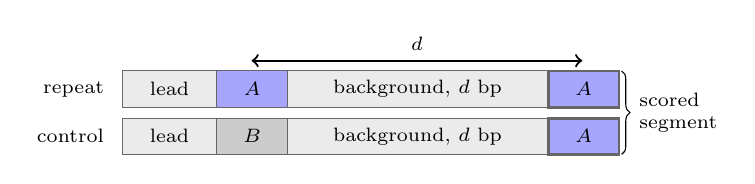
\begin{tikzpicture}[x=1mm,y=1mm,font=\scriptsize,
  box/.style={draw=black!60,minimum height=4.6mm,inner sep=0pt,anchor=west}]
  % repeat window
  \node[anchor=east] at (-1,6) {repeat};
  \node[box,fill=black!8,minimum width=12mm] (l1) at (0,6) {lead};
  \node[box,fill=blue!35,minimum width=9mm] (a1) at (12,6) {$A$};
  \node[box,fill=black!8,minimum width=33mm] (d1) at (21,6) {background, $d$ bp};
  \node[box,fill=blue!35,minimum width=9mm,line width=1pt] (s1) at (54,6) {$A$};
  % control window
  \node[anchor=east] at (-1,0) {control};
  \node[box,fill=black!8,minimum width=12mm] at (0,0) {lead};
  \node[box,fill=black!20,minimum width=9mm] at (12,0) {$B$};
  \node[box,fill=black!8,minimum width=33mm] at (21,0) {background, $d$ bp};
  \node[box,fill=blue!35,minimum width=9mm,line width=1pt] (s2) at (54,0) {$A$};
  \draw[<->,thick] (16.5,9.6) -- node[above] {$d$} (58.5,9.6);
  \node[anchor=west,align=left] at (64.5,3) {scored\\ segment};
  \draw[decorate,decoration={brace,amplitude=3pt}] (63.5,8.3) -- (63.5,-2.3);
\end{tikzpicture}
\caption{The paired windows. Both windows are $C$ tokens long and contain the \emph{same}
final segment $A$ (256\,bp of real hg38). In the repeat window, $A$ also appears $d$\,bp
earlier; in the control window that position holds background $B$. The copy advantage
$\Delta(d)=\mathrm{CE}_{\text{control}}(A)-\mathrm{CE}_{\text{repeat}}(A)$ isolates how much
the model uses the earlier copy.}
\label{fig:protocol}
\end{figure}

\subsection{Task construction}
\label{sec:construction}

\textbf{Design goal.} We want a score that is (i) zero for any model that cannot use
information $d$ bp back, (ii) large for a model that can, and (iii) unaffected by everything
else about the model---its local perplexity, tokenizer, and training data. A single window
cannot achieve (iii), because a model's loss on a segment reflects both recall and ordinary
sequence modeling. We therefore use \emph{paired} windows that differ in exactly one respect.

\textbf{Windows.} For a target distance $d$ and segment length $s=256$\,bp, we choose the
window length $C$ as the smallest power of two with $C \ge 2s+d+64$, so a lead of at least
64\,bp of background precedes the first copy. We sample one contiguous stretch of held-out
genome and split it into four pieces: lead $L$, control piece $B$ ($s$\,bp), distance piece
$D$ ($d$\,bp), and segment $A$ ($s$\,bp). We then build
\begin{align*}
  x^{\text{rep}} &= [\,L;\,A;\,D;\,A\,], &
  x^{\text{ctl}} &= [\,L;\,B;\,D;\,A\,].
\end{align*}
The control window is unmodified contiguous genome; the repeat window replaces $B$ with a
copy of $A$. The final $A$---the scored segment---and the $d$\,bp immediately before it are
identical in both windows. Any difference in the model's loss on the final $A$ must therefore
come from information it carries across at least $d$ bp.

\textbf{Background.} All sequence is drawn from the Basenji/Enformer \emph{test}
intervals~\cite{kelley2018basenji,avsec2021enformer} of GRCh38/hg38, the split that HyenaDNA
and Mnemos-DNA hold out during pretraining. Overlapping intervals are merged into contiguous
blocks and uppercased; we reject windows with $\ge 1\%$ \texttt{N}. Using real genome rather
than random bases keeps inputs in-distribution: a model is never asked to process sequence
statistics it has never seen, so a null result cannot be blamed on distribution shift. Every
window in this paper was drawn from a single contiguous block.

\subsection{Scoring}
\label{sec:scoring}

\textbf{Causal models} are scored by summed next-token cross-entropy over the tokens of the
final $A$. \textbf{Masked models} are scored by masking the \emph{entire} final $A$ and
predicting it in a single forward pass; with the segment fully hidden, the only source of
segment-specific information is the earlier copy, read bidirectionally. In both cases
\begin{equation}
  \Delta(d) \;=\; \frac{1}{s}\Big(\mathrm{CE}\big(A \mid x^{\text{ctl}}\big)
               - \mathrm{CE}\big(A \mid x^{\text{rep}}\big)\Big)
  \quad\text{[nats/bp]}.
\end{equation}
Normalizing by base pairs rather than tokens makes $\Delta$ comparable across tokenizers.
For orientation, a uniform distribution over four bases costs $\ln 4 \approx 1.386$\,nats/bp,
and DNA~LMs reach roughly $1.0$--$1.3$\,nats/bp on held-out human sequence, so $\Delta$ is
bounded above by the model's own control loss: a model that copies $A$ perfectly approaches
that bound, and a model that ignores the first copy scores $0$.

\textbf{Tokenizer alignment.} For $k$-mer or BPE tokenizers, tokenizing the concatenated
string could merge tokens across piece boundaries and make the scored tokens differ between
windows. We instead tokenize each piece separately and concatenate token lists, and we round
piece lengths to a multiple of the model's \texttt{align} (6 for 6-mer models). The final $A$
is thus byte-identical at the token level in both windows. Because the control piece may
tokenize to a different length under BPE, scored spans are located from the end of the window.

\textbf{Statistics.} Each $(d, C)$ point uses $n=128$ independent trials with a random
generator seeded by $(\text{seed}, C, d)$, so every model sees the \emph{same} sequences at a
given point. We report the mean of per-trial $\Delta$ with a 95\% percentile bootstrap
interval (1{,}000 resamples). A point is skipped when $C$ exceeds the model's maximum context
or the run exceeds GPU memory; skips are reported explicitly rather than imputed.

\subsection{Properties and what the score does \emph{not} mean}

\textbf{Conservative by construction.} Inserting $A$ in place of $B$ removes the natural
upstream context of $D$. At very short $d$ this can slightly \emph{hurt} the repeat window,
which is why some models show small negative $\Delta$ at $d=64$ (\S\ref{sec:results}). The
copy advantage is therefore a lower bound on the information a model extracts from the copy;
the foreign control below removes this penalty.

\textbf{Scope.} $\Delta(d)>0$ certifies that a model can retrieve exact earlier content at
distance $d$; it does not certify that the model uses \emph{biological} long-range
dependencies, which are rarely exact copies. Conversely, $\Delta(d)\approx 0$ means that the
model does not use an exact earlier copy at distance $d$ zero-shot, which is a strict
precondition for exploiting repeats and duplications but not for every long-range signal.
We regard \textsc{RecallBench-DNA} as a \emph{necessary-capability} test that complements,
rather than replaces, task benchmarks.

\subsection{Protocol extensions}
\label{sec:extensions}

The construction above tests one specific case: an \emph{exact}, \emph{same-strand} copy,
compared against the \emph{native} genome. Each restriction can be relaxed independently, and
we provide three options that do so while keeping the paired design.

\textbf{Foreign control.} In the default (\emph{native}) control, $B$ is the sequence that
genuinely precedes $D$, whereas the repeat window splices in $A$; the two windows therefore
differ both in \emph{whether} the earlier piece matches $A$ and in \emph{whether} it fits its
surroundings. The \emph{foreign} control replaces $B$ with a 256\,bp segment drawn from an
unrelated genomic location. Both windows then contain an out-of-place piece, and they differ
only in its identity, so $\Delta$ measures recall alone.

\textbf{Diverged repeats.} Real repeats are rarely identical: paralogs, segmental duplications,
and transposable-element copies differ by point substitutions. The \emph{mutate} variant
substitutes each base of the \emph{first} copy independently with probability $p$ (uniformly
among the other three bases). The scored final copy is unchanged, so $\Delta$ measures how much
a model can still exploit a copy that diverges from the target at rate $p$.

\textbf{Inverted repeats.} DNA is double-stranded, and a sequence frequently recurs as its
reverse complement (inverted repeats, hairpins, transposons inserted on the opposite strand).
The \emph{revcomp} variant uses the reverse complement of $A$ as the first copy. A model with
strand-aware recall can exploit it; a model that only matches forward strings cannot.

\textbf{Pairing across options.} Randomness for an option (substitution positions, the foreign
segment) is drawn from a separate generator seeded by $(\text{seed}, C, d, 1)$. The lead,
background, and segment for a given $(\text{seed}, C, d)$ are therefore identical under every
option, so differences between options are themselves paired comparisons, and the default
options reproduce the original windows exactly.

\subsection{Software package}
\label{sec:impl}

\textsc{RecallBench-DNA} is distributed as a pip-installable Python package,
\texttt{recall-bench}, with a minimal core (PyTorch, NumPy, PyYAML) and optional extras for
Hugging Face models and data preparation. It is designed so that evaluating a new model takes
a few lines and no knowledge of the benchmark's internals:

\begin{small}
\begin{verbatim}
import recall_bench as rb
m = rb.CallableModel(logits_fn=net, tokenize=enc,
                     causal=True, max_ctx=131072)
rows = rb.evaluate(m, distances=[64, 1024, 65536],
                   variant="mutate", mut_rate=0.05)
\end{verbatim}
\end{small}

\noindent Any callable that maps token ids to logits can be wrapped, masked LMs are supported
via a mask token, and any Hugging Face causal or masked LM can be loaded by identifier. A
command-line tool (\texttt{recall-bench prepare|run|run-hf|report}) builds the held-out
background, runs sweeps, and prints result tables. A packaged registry lists each released
model's family, identifier, maximum context, and tokenizer alignment; adding a model is one
line. Models are downloaded only when tested and can be deleted afterwards, so the full study
fits on a laptop disk. Every trial is checkpointed atomically; an interrupted run resumes by
replaying the random stream without model calls, producing results bit-identical to an
uninterrupted run. A CPU-only test suite checks the protocol against two reference models: a
model that ignores context must score exactly $\Delta=0$, and a $k$-gram induction model that
copies forward must score highly on exact repeats, less on mutated ones, and near zero on
reverse-complement ones. All results in this paper were produced on one NVIDIA RTX~5060
Laptop GPU (8\,GB) in bf16.

% ---------------------------------------------------------------------------------------------
\section{Experimental Setup}
\label{sec:setup}

\textbf{Models.} We evaluate ten released DNA~LM checkpoints, grouped by whether they contain
an explicit content-addressed memory (Table~\ref{tab:models}).
\emph{HyenaDNA}~\cite{nguyen2023hyenadna}: tiny-1k, small-32k, medium-450k, and large-1m.
\emph{Caduceus}~\cite{schiff2024caduceus}: the Ph and PS variants at 131\,kbp.
\emph{Mnemos-DNA}~\cite{balyan2026mnemos}: four $\sim$2.3M-parameter, single-nucleotide arms
trained on hg38 at 131\,kbp context with matched token budgets---pure gated delta-rule
linear attention (KDA; D01), KDA with windowed local attention (D02), KDA with a per-layer
$k$-mer fast-weight memory keyed by the exact preceding 8-mer (D06, ``Mnemos-DNA''), and D06
with an added local-attention block and length curriculum (D07, ``Mnemos-DNA-C''). D01 and D02
are the matched controls for the memory. Masked models (Caduceus) use the masked scoring rule;
all others are causal.

\begin{table}[t]
\centering
\caption{Evaluated checkpoints. ``Ctx'' is the advertised maximum context.}
\label{tab:models}
\footnotesize
\setlength{\tabcolsep}{4pt}
\begin{tabular}{@{}llrl@{}}
\toprule
Model & Mechanism & Ctx & Scoring \\
\midrule
HyenaDNA (4 sizes)  & implicit long conv.       & 1K--1M & causal \\
Caduceus-Ph/PS      & bidir.\ Mamba (RC-equiv.) & 131K   & masked \\
Pure KDA (D01)      & gated delta rule          & 131K   & causal \\
KDA+Local (D02)     & + windowed attention      & 262K   & causal \\
Mnemos-DNA (D06)    & + 8-mer fast-weight mem.\ & 131K  & causal \\
Mnemos-DNA-C (D07)  & + local attn., curriculum & 131K   & causal \\
\bottomrule
\end{tabular}
\end{table}

\textbf{Sweep.} $d \in \{64, 256, 1\text{K}, 4\text{K}, 16\text{K}, 64\text{K}, 256\text{K}\}$\,bp,
giving window lengths $C$ from 2{,}048 to 524{,}288 tokens; $s=256$\,bp; $n=128$ trials per
point; seed 0. The smallest window (2{,}048) exceeds HyenaDNA-tiny's 1{,}024-token limit, so
that model is skipped at every distance and reported only for completeness.

% ---------------------------------------------------------------------------------------------
\section{Results}
\label{sec:results}

\begin{figure*}[t]
\centering
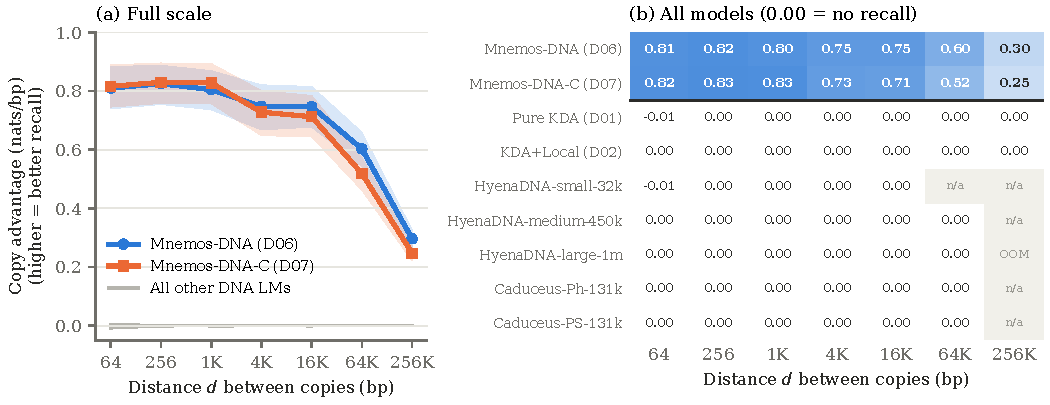
\includegraphics[width=\textwidth]{../figures/recall_vs_distance.pdf}
\caption{Copy advantage versus distance between copies. (a) Full scale: the two models with a
$k$-mer fast-weight memory retain most of their recall to 16\,kbp and remain clearly
positive at 256\,kbp, twice their 131\,kbp training context. Every other model lies on the
zero line. (b) Copy advantage (nats/bp) for every model and distance; darker
cells mean stronger recall, n/a marks distances beyond a model's context. No model without
the memory exceeds $0.0021$\,nats/bp at any distance.}
\label{fig:main}
\end{figure*}

\begin{table*}[t]
\centering
\caption{Copy advantage $\Delta(d)$ in units of $10^{-2}$\,nats/bp (mean over 128 trials).
\textbf{Bold}: memory models, 95\% CI excludes zero. $^*$: CI excludes zero for a model
without memory; positive such effects are $\le 0.14\times10^{-2}$, two to three orders of
magnitude below the memory models, and significant negatives occur only at $d=64$
(\S\ref{sec:benchmark}, conservative construction). $\times$: window exceeds the model's maximum
context. \textsc{oom}: exceeds 8\,GB GPU memory.}
\label{tab:results}
\small
\begin{tabular}{@{}lrrrrrrr@{}}
\toprule
& \multicolumn{7}{c}{Distance $d$ between copies (bp)} \\
\cmidrule(l){2-8}
Model & 64 & 256 & 1K & 4K & 16K & 64K & 256K \\
\midrule
\csname @@input\endcsname ../figures/recall_table.tex
\bottomrule
\end{tabular}
\end{table*}

\textbf{Finding 1: released long-context DNA~LMs do not use an exact earlier copy.}
Across HyenaDNA-small, -medium, and -large and both Caduceus variants, the copy advantage never
exceeds $0.0021$\,nats/bp (Table~\ref{tab:results}, Fig.~\ref{fig:main}b). For scale, a
model that recovered even 1\% of the segment's information from the first copy would score
$\approx 0.01$\,nats/bp, about five times the largest value observed. Some points are
statistically distinguishable from zero---for example HyenaDNA-large at 1\,kbp
($+0.0014$, CI $[0.0004, 0.0026]$)---but these effects amount to $\approx 0.35$\,nats over
the whole 256\,bp segment and are best read as weak local carry-over, not retrieval. The
absence of recall holds at distances far inside the advertised context: HyenaDNA-large-1m
shows $|\Delta| < 10^{-4}$ at 64\,kbp, a distance it nominally covers sixteen times over.

\textbf{Finding 2: a fixed-size recurrent state is not enough, with or without local
attention.} The matched Mnemos-DNA controls isolate architecture from training data and
budget. Pure KDA (D01) and KDA with windowed local attention (D02) match the released
baselines: $|\Delta| < 0.006$ at every distance. Adding local attention does not help even at $d=64$. This is consistent with the copying
gap of fixed-state models reported in NLP~\cite{jelassi2024repeat,arora2024zoology}, and
shows that it carries over to DNA.

\textbf{Finding 3: content-addressed memory produces strong, long-range recall.} Adding the
8-mer fast-weight memory (D06) changes the picture entirely. $\Delta$ is $0.80$--$0.82$
nats/bp up to 1\,kbp---recovering roughly $210$\,nats over each 256\,bp segment---declines
gently to $0.75$ at 16\,kbp and $0.60$ at 64\,kbp, and remains $0.30$ (CI $[0.26,0.33]$) at
256\,kbp. D07 behaves almost identically up to 1\,kbp and decays slightly faster beyond
4\,kbp ($0.52$ at 64\,kbp, $0.25$ at 256\,kbp). Since the only difference between D01 and D06
is the memory, the recall is attributable to it.

\textbf{Finding 4: recall extrapolates beyond the training context.} Both memory models were
trained on 131\,kbp windows, yet at $d=256$\,kbp, evaluated in 524\,kbp windows, they retain
$30$--$36\%$ of their peak copy advantage. Among released baselines, none could be
evaluated at this distance on an 8\,GB GPU: Caduceus and HyenaDNA-medium exceed their
maximum context, and HyenaDNA-large runs out of memory.

% ---------------------------------------------------------------------------------------------
\section{Why This Benchmark Is Useful}
\label{sec:usefulness}

\textbf{For model developers: a cheap, honest check on context claims.} A full sweep for one
model takes between minutes and a few hours on a laptop GPU, with no training. Our results
show that an advertised context length can differ from usable recall by three orders of
magnitude; reporting $\Delta(d)$ alongside context length would make such claims verifiable.

\textbf{For architecture research: an isolating diagnostic.} Because the score is paired,
zero-shot, and distance-resolved, it attributes recall to architecture rather than to
fine-tuning protocol. In our matched comparison, it separates models that differ by a single
component (D01 vs.\ D06) with every memory-model point lying 16--23 standard errors above zero. It is a natural
regression test for new memory mechanisms, state-size scaling, or hybrid designs.

\textbf{For genomics applications: a prerequisite for repeat-aware modeling.} Segmental
duplications, gene families, transposable elements, and tandem repeats make exact or
near-exact recurrence pervasive in eukaryotic genomes~\cite{dekoning2011repeats}. Tasks that
exploit such structure---variant interpretation in paralogous regions, repeat annotation, or
assembly-aware modeling---require that a model can relate a position to an earlier copy.
\textsc{RecallBench-DNA} tests that prerequisite directly.

\textbf{For benchmarking practice: complementary to task suites.} Task benchmarks answer
``is the model useful for $X$?'' This benchmark answers ``does the model have the mechanism
that long-range $X$ would need?'' When a long-context model underperforms on a long-range
task, a near-zero $\Delta$ points to the backbone; a large $\Delta$ points to the task
protocol or head.

\textbf{For accessibility.} The entire study, including 1\,Mbp-class checkpoints, runs on a
single 8\,GB consumer GPU, with models fetched and deleted one at a time. This lowers the
barrier for groups without datacenter hardware to audit published models.

% ---------------------------------------------------------------------------------------------
\section{Limitations and Future Work}
\label{sec:limitations}

\textbf{Copy types.} The protocol extensions (\S\ref{sec:extensions}) cover substitutions
and reverse complements, but not insertions and deletions, which shift the alignment between
the copies; indel-bearing repeats and tandem (adjacent, $d=0$) repeats are natural next
variants. \textbf{Exact recall is not biological long-range modeling.} Enhancer--promoter
interactions and other long-range signals are not copies, so a high $\Delta$ is necessary but
not sufficient for them; pairing this benchmark with task suites such as the Genomics
Long-Range Benchmark~\cite{trop2024lrb} remains essential. \textbf{Coverage.} We report nine
evaluable checkpoints. The package already supports the Nucleotide Transformer, DNABERT-2,
GENA-LM, GENERator, and Evo~2, and a text-LM positive control
(Pythia~\cite{biderman2023pythia}, Mamba, RWKV, GLA, and DeltaNet on
WikiText-103~\cite{merity2017wikitext}); these runs are in progress and not reported here.
Protocol extensions were run up to 64\,kbp. \textbf{Hardware ceiling.} Distances beyond
256\,kbp, and some models at 256\,kbp, require more than 8\,GB of GPU memory.
\textbf{Single segment length, seed, and genome.} We fix $s=256$\,bp, seed 0, and the human
genome; every point averages 128 independent windows, and the package accepts any
background (e.g.\ other species) and segment length, but we have not yet studied these axes.
\textbf{Potential conflict
of interest.} The Mnemos-DNA models are from the same author as this benchmark, which was
originally developed as an evaluation probe for them. To mitigate this, the protocol, code,
and all per-trial results are public, every model is evaluated by the identical procedure on
identical sequences, and the comparisons that carry the central architectural claim (D01 and
D02 vs.\ D06) are among matched in-house models.

\section{Conclusion}

Long context is a property of the input; recall is a property of the model. We introduced
\textsc{RecallBench-DNA}, a zero-shot, paired, distance-resolved benchmark that measures
whether a DNA language model can use an exact earlier copy of a sequence. On nine released
checkpoints it reveals a sharp split: widely used long-context models show no meaningful
recall at any distance, while models with a content-addressed $k$-mer memory recall strongly
up to 256\,kbp. We hope the benchmark becomes a routine companion to context-length claims
and a diagnostic for the next generation of long-range genomic models.

\section*{Availability}
Code, model registry, and all per-trial results:
\url{https://github.com/B4K2/recall-bench}. Mnemos-DNA weights:
\url{https://huggingface.co/B4K2xx/Mnemos-DNA}.
